\documentclass[border=3pt]{standalone}
\usepackage[T1]{fontenc}
\usepackage[utf8]{inputenc}
\usepackage{lmodern}
\usepackage{amsmath,amssymb}
\usepackage{xcolor}
\usepackage{tikz}
\usepackage{fontawesome5}
\usepackage{ragged2e}
\usetikzlibrary{shapes,shapes.geometric,shapes.misc,arrows.meta,positioning,
                calc,fit,backgrounds,decorations.pathreplacing,
                decorations.markings,patterns,chains}
\usetikzlibrary{decorations.pathreplacing,decorations.markings}
\definecolor{primary}{HTML}{1A5276}
\definecolor{secondary}{HTML}{2E86C1}
\definecolor{accent}{HTML}{E74C3C}
\definecolor{lightbg}{HTML}{EBF5FB}
\definecolor{defbg}{HTML}{FDF2E9}
\definecolor{greenhl}{HTML}{27AE60}
\definecolor{purplehl}{HTML}{8E44AD}
\definecolor{goldhl}{HTML}{B7950B}
\definecolor{tealhl}{HTML}{117A65}
\definecolor{codebg}{HTML}{F4F6F7}
\definecolor{neutral}{HTML}{707B7C}
\definecolor{dom1}{HTML}{1F618D}
\definecolor{dom2}{HTML}{117864}
\definecolor{dom3}{HTML}{6C3483}
\definecolor{dom4}{HTML}{922B21}
\definecolor{dom5}{HTML}{B7950B}
% --- carried over from ccna.sty so figures match the book exactly
\tikzset{
  dev/.style={rounded corners=3pt, draw=#1, fill=#1!8, text=#1!45!black,
              line width=0.9pt, minimum width=1.45cm, minimum height=1.05cm,
              align=center, font=\scriptsize\bfseries, inner sep=2pt},
  wirestyle/.style={line width=0.9pt, neutral!75},
  xconn/.style={line width=0.9pt, neutral!75, dash pattern=on 2.5pt off 2pt},
}

\newcommand{\Rtr}[3]{\node[dev=dom3] (#1) at #2 {\faIcon{route}\\#3};}
\newcommand{\Sw}[3]{\node[dev=dom2] (#1) at #2 {\faIcon{sitemap}\\#3};}
\newcommand{\Msw}[3]{\node[dev=dom3] (#1) at #2 {\faIcon{layer-group}\\#3};}
\newcommand{\Host}[3]{\node[dev=neutral] (#1) at #2 {\faIcon{desktop}\\#3};}
\newcommand{\Lap}[3]{\node[dev=neutral] (#1) at #2 {\faIcon{laptop}\\#3};}
\newcommand{\Srv}[3]{\node[dev=dom1] (#1) at #2 {\faIcon{server}\\#3};}
\newcommand{\Ap}[3]{\node[dev=dom5] (#1) at #2 {\faIcon{wifi}\\#3};}
\newcommand{\Wlc}[3]{\node[dev=dom5] (#1) at #2 {\faIcon{broadcast-tower}\\#3};}
\newcommand{\Fw}[3]{\node[dev=dom4] (#1) at #2 {\faIcon{shield-alt}\\#3};}
\newcommand{\Cld}[3]{\node[dev=neutral] (#1) at #2 {\faIcon{cloud}\\#3};}
\newcommand{\Phone}[3]{\node[dev=dom5] (#1) at #2 {\faIcon{phone-alt}\\#3};}
\newcommand{\Prn}[3]{\node[dev=neutral] (#1) at #2 {\faIcon{print}\\#3};}

% A link. The optional argument takes tikz options (e.g. xconn for a
% trunk drawn dashed); the fourth argument labels the link.
\newcommand{\wire}[4][wirestyle]{%
  \draw[#1] (#2) -- node[font=\tiny, text=neutral!85!black, fill=white,
                          inner sep=1.2pt, midway] {#4} (#3);}
\newcommand{\plainwire}[3][wirestyle]{\draw[#1] (#2) -- (#3);}


\newenvironment{topology}[1][]
  {\begin{center}\begin{tikzpicture}[font=\scriptsize,#1]}
  {\end{tikzpicture}\end{center}}


\newcommand{\cmd}[1]{\texttt{\small #1}}
\newcommand{\term}[1]{\textbf{\textcolor{primary}{#1}}}
\newcommand{\chref}[1]{Chapter~\ref{ch:#1}}
\newcommand{\ccnafitw}[1]{#1}
\providecommand{\thefigure}{}
% --- progressive builds
\newcount\buildlevel \buildlevel=99
% \stepvis{n}{..} appears from level n onward; \steponly{n}{..} at
% level n alone, which is how a caption is swapped rather than
% accumulated as the build advances.
\newcommand{\stepvis}[2]{\ifnum#1>\buildlevel\relax\else#2\fi}
\newcommand{\steponly}[2]{\ifnum#1=\buildlevel #2\fi}
\begin{document}
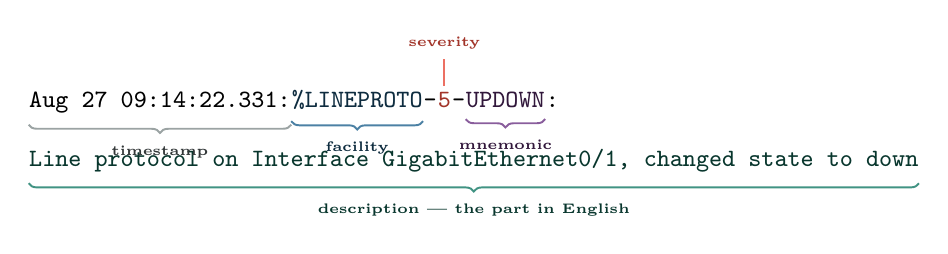
\begin{tikzpicture}[font=\scriptsize]
  % Each part of the message is its own node, chained left to right, so
  % the braces below can attach to real anchors instead of to guessed
  % character positions.
  \tikzset{
    seg/.style={font=\ttfamily\small, inner xsep=0pt, inner ysep=2pt,
                anchor=base west},
    br/.style={decorate, decoration={brace, amplitude=3pt, mirror},
               line width=0.7pt, #1},
    cap/.style={font=\tiny\bfseries, text=#1!45!black, align=center,
                anchor=north}}

  \node[seg]                        (ts)  at (0,0)             {Aug 27 09:14:22.331:~};
  \node[seg, text=dom1!45!black]    (fac) at (ts.base east)    {\%LINEPROTO};
  \node[seg]                        (d1)  at (fac.base east)   {-};
  \node[seg, text=accent!70!black]  (sev) at (d1.base east)    {5};
  \node[seg]                        (d2)  at (sev.base east)   {-};
  \node[seg, text=dom3!45!black]    (mne) at (d2.base east)    {UPDOWN};
  \node[seg]                        (cl)  at (mne.base east)   {:};

  \node[seg, text=dom2!45!black, anchor=north west] (desc)
      at ([yshift=-0.30cm]ts.south west)
      {Line protocol on Interface GigabitEthernet0/1, changed state to down};

  \draw[br=neutral!70] ([yshift=-2pt]ts.south west) -- ([yshift=-2pt]ts.south east);
  \node[cap=neutral] at ([yshift=-6pt]ts.south) {timestamp};

  \draw[br=dom1!80] ([yshift=-2pt]fac.south west) -- ([yshift=-2pt]fac.south east);
  \node[cap=dom1] at ([yshift=-6pt]fac.south) {facility};

  \draw[br=dom3!80] ([yshift=-2pt]mne.south west) -- ([yshift=-2pt]mne.south east);
  \node[cap=dom3] at ([yshift=-6pt]mne.south) {mnemonic};

  % Severity is one character wide, so it gets a leader upward instead
  % of a brace it would dwarf.
  \draw[accent!80, line width=0.7pt] (sev.north) -- ++(0,0.34)
      node[font=\tiny\bfseries, text=accent!70!black, anchor=south] {severity};

  \draw[br=dom2!80] ([yshift=-2pt]desc.south west) -- ([yshift=-2pt]desc.south east);
  \node[cap=dom2] at ([yshift=-6pt]desc.south) {description --- the part in English};
\end{tikzpicture}
\end{document}
